\documentclass[11pt,a4paper]{article}
\usepackage[utf8]{inputenc}
\usepackage{amsmath}
\usepackage{amsfonts}
\usepackage{amssymb}
\usepackage{ngerman}
\usepackage{graphicx}
\usepackage{geometry}
\usepackage{setspace}
\usepackage{cite}
\usepackage{url}
\usepackage{caption}
\usepackage{tikz}
\usepackage{colortbl}
\usepackage{sidecap}
\usepackage{wrapfig}

\overfullrule=0pt

\begin{document}

\tableofcontents
\newpage

\setstretch{1.3}

\section{Einleitung}
Das menschliche Gehör hat die Fähigkeit komplexe akustische Signale zu verarbeiten und zu interpretieren. Für eine Person ist es kein Problem aus einer Vielzahl von unterschiedlichen Geräuschen eine bestimmte Information zu gewinnen und auf diese zu reagieren. Dabei werden rein mechanische Schwingungen der Luft in abstraktere Informationen umgewandelt und vom Hörzentrum interpretiert, sodass aufeinander folgende Laute beispielsweise als menschliche Sprache erkannt und verstanden werden können. Dabei ist es sehr robust gegenüber Störfaktoren, wie Hintergrundgeräusche oder leise Töne, so werden Laute, auf die man sich konzentriert bis zu drei mal lauter wahrgenommen (Cocktail-Party-Effekt).\\
Die Fähigkeit aus einem komplexen Signal einzelne Features zu extrahieren, ist ein schwer zu erreichendes Ziel für die Informatik, da die zugrundeliegenden Audiodaten kaum formal erfassbaren Regeln unterliegen, die für Algorithmen dafür benutzt werden könnten abstraktere Informationen zu gewinnen, so sind Audiodaten meist sehr komplex und verrauscht.\\
Neben der Wahrnehmung von Sprache und Umweltgeräuschen kann der Mensch Musik wahrnehmen, wobei Musik die besondere Funktion hat Emotionen auszudrücken und zu erzeugen. Dabei können sich die erzeugten Emotionen stark unterscheiden und sind von vielen Faktoren abhängig. Zu diesen Faktoren gehören die Harmonik, die Rhythmik, die Melodik, sowie subjektive Faktoren, wie die Hörerwartung des Hörers und dessen musikalische Prägung.\\
Der Versuch die in der Musik erzeugten Emotionen zu berechnen oder zu klassifizieren wird ``Music Emotion Recognition'' genannt. Grade in den letzten Jahren wurde die Forschung auf diesem Gebiet verstärkt, vor allem mit der Motivation Musik nach Emotionen sortieren und anbieten zu können. Dabei werden nach den modernsten Methoden verschiedene Lowlevel und Highlevel Features aus der Musik extrahiert, um diese dann mit Machine Learning Algorithmen zu klassifizieren. Dafür müssen große Mengen von Musik von Menschen klassifiziert werden, was vor allem durch die Subjektivität der Hörer erschwert wird.\\
Die emotionalen Eigenschaften von Musik werden längst in Multimedialen Inhalten genutzt, um die Wirkung der Medien zu verstärken. So wird Musik bewusst eingesetzt, um Filme und Spiele anzureichern.\\
Andersherum sind Videos und Animationen eine Möglichkeit Musik zu untermalen. So werden vor allem in der kommerziellen Musikproduktion zahlreiche Musikvideos produziert. Auch haben viele moderne Musikplayer eine eingebaute Visualisierung, die sich passend zur Musik verändert. Diese Visualisierung basiert meistens auf einer Analyse der Musik, die keine tiefer gehenden Informationen aus der Musik zieht. Die Visualisierung ist eher willkürlich, als der Musik nachempfunden.\\
An dieser Stelle möchte ich ansetzen und untersuchen auf welche Art und Weise eine Visualisierung der Musik durchgeführt werden kann, sodass aus der Musik eine Visualisierung generiert werden kann, die eine intuitive Verbindung zu den Emotionen des Hörers hat.

\subsection{Unterschiede zu anderen Visualisierungen}
% andere Visualizer keine tiefere Informationsverarbeitung
Im Folgenden möchte ich auf die heutigen Möglichkeiten der Visualisierung eingehen und zeigen, wie sich diese von dem hier beschriebenen Projekt unterscheiden. Die heutigen Visualisierungen kann man in drei grobe Gebiete einteilen.\\
% Standard Visualisierungen
Das erste dieser Gebiete schließt die Visualisierungen der bekannten Audioplayer ein. Diese haben den Anspruch zu jeder beliebigen Musik eine passende Visualisierung zu schaffen und dabei wenig Ressourcen zu verbrauchen. Auch müssen sie ohne externe Information auskommen, die helfen könnte eine bessere Visualisierung zu erschaffen. Der Nachteil dieser Bedingungen ist eine relativ technische Interpretation der Musik, die dazu führt, dass auf unterschiedliche Emotionen, die in der Musik auftauchen nicht eingegangen wird. Sie funktionieren, indem entweder die Lautstärke der Musik Einfluss auf die Visualisierung nimmt oder die Musik über eine FFT (siehe Grundlagen) in Frequenzbänder übersetzt wird, die dann einzeln in die Visualisierung eingehen. Diese Art der Visualisierung wird beispielsweise bei der MilkDrop-Visualisierung oder beim bekannten Musikplayer iTunes verwendet.\\
% Visualisierung selber machen (Adobe After Effects)
Die zweite Variante wird vor allem in Einzelfällen und zunehmend für elektronische Musik verwendet. Hierbei wird die Visualisierung speziell für ein Musikstück von Hand umgesetzt. Hierbei werden wie auch bei der ersten Variante technische Aspekte der Musik mit einbezogen, um den Bezug zwischen Musik und Visualisierung zu erschaffen. Dazu werden spezielle Programme, wie Adobe After Effects, verwendet. Der große Vorteil dieser Variante ist der, dass man eine einzigartige Visualisierung erzeugt, die speziell auf dieses Lied angepasst sein kann. Man kann so die wahrscheinlich besten Ergebnisse erzielen. Der Nachteil ist, dass für ein neues Lied eine neue Visualisierung erschaffen werden muss.\\
% Visualisierung sehr nahe an Noten
Die dritte Variante der Visualisierungen ist heute nur noch wenig populär und basiert darauf, dass externe Informationen für die Visualisierung bereit gestellt werden. Die 1985 vorgestellte ``Music Animation Machine'' orientiert sich an MIDI Noten, die passend zur laufenden Musik bereitgestellt sind. Der Zusammenhang mit der Musik ist damit unmittelbar hergestellt, allerdings ist die Interpretation der Musik damit auch auf einer sehr technischen Ebene, da Emotionen, die durch die Musik erzeugt werden nicht in die Visualisierung einfließen.\\
Das Ziel dieser Arbeit ist es Algorithmen zu entwickeln und zu beschreiben, die aus einem Audiosignal eine Visualisierung entwickeln, die sich passend zur empfundenen Stimmung entwickelt. Dafür muss man sich damit beschäftigen, wie menschliche Emotionen auf berechenbare Modelle abgebildet werden können und wie diese extrahierte Information dann in eine Visualisierung einfließen kann.

\section{Grundlagen}
Im Folgenden sollen kurz Grundlagen erläutert werden, die helfen sollen die implementierten Algorithmen zu verstehen.
\subsection{Tonleitern}
Um zu verstehen, welche Musik positive, freudige  oder negative, traurige Emotionen hervorruft, soll an dieser Stelle kurz auf die musikalischen Grundlagen der Tonleitern eingegangen werden.
Eine Tonleiter ist eine Menge von Tönen, die einen Grundton besitzt. Es gibt unterschiedliche Tonleitern, mit denen unterschiedliche Emotionen verbunden werden. In den folgenden Bildern sind Klaviaturen zu sehen, auf denen die Töne der C Tonleitern markiert sind.
\begin{figure}[ht]
\begin{center}
\begin{tabular}{c c c}
C Dur & \hspace{15pt} C Reines Moll & \hspace{15pt} C Harmonisches Moll \\
\includegraphics[scale=1.2]{res/images/keyboard_dur} & \hspace{15pt} \includegraphics[scale=1.2]{res/images/keyboard_rein_moll} & \hspace{15pt} \includegraphics[scale=1.2]{res/images/keyboard_harm_moll}
\end{tabular}
\caption[C Tonleitern]{Die C Tonleitern}

\end{center}
\end{figure}

Der Grundton dieser Tonleitern ist das C. Es befindet sich ganz links auf der Klaviatur. Entscheidend für die Wirkung einer Tonleiter ist der Abstand der Tonleitertöne zum Grundton. Wie man sieht ist der dritte Ton (die Terz) über dem Grundton bei beiden Moll-Tonleitern einen Halbtonschritt niedriger, sowie der sechste Ton (die Sexte). Man spricht hierbei von der kleinen Terz und der kleinen Sexte. Der siebte Ton (die Septime oder Septe) ist beim reinen Moll eine kleine Septime, während sie beim harmonischen Moll eine große Septime ist, gleich der Dur-Tonleiter. Die große Septime wird auch Leitton genannt.\\
Neben dem reinen und dem harmonischen Moll existiert noch das melodische Moll, das sich beim aufwärts und abwärts spielen unterscheidet. Beim aufwärts spielen wird die Sexte und die Septime wie in der Dur-Tonleiter gespielt, beim abwärts spielen wie im reinen Moll. Diese Tonleiter wird im Folgenden nicht weiter behandelt. Weiterhin existieren noch die sogenannten Kirchentonleitern, sowie zahlreiche Blues und Jazz Tonleitern, die meistens ``Scalen'' genannt werden und in denen häufig die kleine Septime wie im reinen Moll gespielt wird.\\
Da das reine Moll und das Harmonische Moll sich von der Dur Tonleiter in der Terz und in der Sexte unterscheiden, könnte man diese Töne in die Approximation der Stimmung des Musikstückes mit einfließen lassen. Die Septime ist weniger gut zu verwenden, da sie im harmonischen Moll als große Septime (wie in der Dur-Tonleiter) und im reinen Moll als kleine Septime vorkommt. Auch wird die kleine Septime sehr häufig in eher positiv freudigen Blues Stücken verwendet.

%\subsubsection{Loudness of Music / Decibel}

\subsection{DCT/DFT/FFT}
% Was ist die DCT / FFT
Die Diskrete Kosinus Transformation (engl. Discrete Cosine Transformation; kurz DCT) ist eine Transformation, die es erlaubt, Werte, die zeitdiskret kodiert sind, in den Frequenzbereich zu transformieren. Wird beispielsweise eine Sinusschwingung mit 440 Hertz in den Frequenzbereich transformiert, so ist der einzige Ausschlag im Frequenzbereich die Frequenz von 440 Hertz. Die Werte im Frequenzbereich werden als Koeffizienten von Kosinusfunktionen dargestellt. Diese Kosinusfunktionen sind unterschiedlich gestreckt, um die verschiedenen Frequenzen abbilden zu können.\\
% Varianten von DCT / FFT
Von der DCT gibt es die Varianten I - VIII von denen die Varianten I - IV praktischen Einsatz finden. Neben der DCT existiert auch die Diskrete Fourier Transformation (kurz DFT), die Frequenzen als Koeffizienten von Kosinus und Sinusfunktionen darstellt. Für die DFT gibt es eine optimierte Implementierung, die sogenannte Schnelle Fourier Transformation (engl. Fast Fourier Transformation; kurz FFT), die es erlaubt eine DFT mit logarithmischer Komplexität durchzuführen.\\
% Anwendungsgebiete
Anwendung findet die DCT bei der verlustbehafteten Audio- und Bildkompression. Für die Analyse des Spektrums eines Musikausschnittes bietet sich vor allem, dank ihrer besseren Laufzeit, die FFT an \cite[S. 20 f.]{lerch2012introduction}.

%\subsubsection{Lautstärke}
% TODO

\section{Analyse}

\subsection{Zielsetzung}
% Musik gerecht visualisieren
Ziel dieser Arbeit ist es herauszuarbeiten, wie ein Programm umgesetzt werden kann, das eine Visualisierung entwickelt, die eine enge Verbindung zur Musik aufweist. Dazu soll eine tiefere Interpretation der Musik erfolgen, deren Ergebnisse dann benutzt werden, um eine Darstellung zu generieren, die die Empfindungen des Hörers bestärken.\\
% Was braucht man für Visualisierung? Emotionen/Events
Bei dieser Aufgabenstellung stellt sich die Frage welche Informationen von der Musik benötigt werden. Da Musik zeitlich abläuft, empfiehlt es sich auf Zeitpunkte in der Musik einzugehen, die eine besondere Relevanz haben. So gibt es Rhythmuselemente, die man unmittelbar beim Hören wahrnimmt, aber auch Events, die weniger häufig auftreten, wie Wechsel von Abschnitten des Songs. Neben diesen zeitlich positionierbaren Events gibt es Informationen, die sich stetig über den Song entwickeln, wie die gespielten Akkorde oder die Lautstärke.\\
Auch sind die empfundenen Emotionen während des Stückes ein interessanter Aspekt, der die Visualisierung anreichern könnte.
% Wie kann man sie ermitteln?
Wenn Emotionen zur Visualisierung genutzt werden sollen, so stellen sich einige Fragen. Auf welche Art können Emotionen ermittelt werden oder welche Features der Musik lassen sich nutzen, um in eine Approximation der empfundenen Stimmung einzugehen?\\
% Wie kann man sie modelieren?
Wie lassen sich Stimmungen oder Emotionen in digitalen Systemen darstellen und welche Darstellung eignet sich für eine Visualisierung? Sollte man versuchen Emotionen zu Klassifizieren oder durch kontinuierliche Werte beschreiben?\\
% Wie kann man sie visualisieren?
Wenn man diese Fragestellungen gelöst hat, so ist weiter zu klären, welche Visualisierung für die ermittelten Daten als passend empfunden wird und wie man diese umsetzt.\\
% Wie kann man testen, ob die Visualisierung als passend empfunden wird?
Als Letztes möchte ich herausstellen, dass auch das Testen der Visualisierung eine Herausforderung darstellt, da die Subjektivität des Hörers ein einheitliches Ergebnis erschwert und die Problematik nicht formal erfassbar zu seien scheint. Die Beantwortung dieser Fragen soll Thema dieser Arbeit sein, sowie die Beschreibung einer prototypischen Umsetzung. 

\subsection{Anforderungen}
Im folgenden werden Anforderungen beschrieben, die an den Quelltext des Prototypen, sowie dessen Resultat gestellt werden.

\subsubsection{Funktionale Anforderungen}
Da der Fokus dieser Arbeit eher auf der Umsetzung von einer Visualisierung liegt, als auf der Interaktion mit dem User gibt es nur wenige funktionale Anforderungen. So wurde beispielsweise auf die Implementierung einer GUI, mit der man die Visualisierung steuern könnte, verzichtet. Im Folgenden soll trotzdem die Funktionsweise des Prototypen beschrieben sein.\\
Die Visualisierung sollte sich mit Angabe einer Audiodatei starten lassen. Dabei sollten unterschiedliche gängige Audioformate, wie wav oder mp3, unterstützt werden, die automatisch erkannt und richtig geladen werden.\\
Als optionale Interaktionsmöglichkeit mit dem Programm könnte die Perspektive bzw. die Kameraposition durch Tastatureingaben und Mausbewegungen des Benutzers verändert werden.\\
Wichtig ist auch, das sich der Prototyp während der Visualisierung beenden lässt.\\
Als weniger wichtig wird angesehen, dass der Prototyp für unterschiedliche Betriebssysteme kompatibel ist. Er wird für die Linux Umgebung entwickelt.

\subsubsection{Nicht funktionale Anforderungen}
Wie in der Zielsetzung schon behandelt, soll die Visualisierung die durch die Musik empfundenen Emotionen bekräftigen. Dazu soll die Musik analysiert werden.\\
Die Analyse der Musik sollte performant implementiert sein, sodass kein längeres Warten auf die Ergebnisse zu spüren ist. Dazu sollen aufwendige Berechnungen, wie beispielsweise eine Spektrumsanalyse nicht mehrfach durchgeführt werden, die Algorithmen effizient implementiert werden und wo dies schwierig ist sollte auf optimierte Software-Bibliotheken zurückgegriffen werden. Auf Optimierung durch Multithreading oder Multiprocessing wird aus Zeitgründen verzichtet.\\
Weiterhin sollten Programmabstürze abgefangen und durch verständliche Fehlermeldungen ersetzt werden. Beispielsweise durch fehlende oder fehlerhafte Audiodateien.\\
Neben den Anforderungen an die Bedienbarkeit des Prototypen existieren Anforderungen, die die Programmierung direkt betreffen. Um unterschiedliche Visualisierungen zu generieren, ist es sinnvoll ein modulares System zu konstruieren, indem unterschiedliche Visualisierungen austauschbar realisiert werden können. Auch andere Bereiche, wie die Analyse der Musik kann man gut mit unabhängigen Modulen realisieren, die die einzelnen Verarbeitungsschritte der Analyse umsetzen. Ein weiterer Vorteil eines modularen Systems ist, dass es einfach erweitert werden kann, indem neue Module hinzugefügt werden.

\subsection{Verwendete Sprachen / Bibliotheken}

\subsubsection{Programmiersprachen}
Für die Umsetzung des Prototypen wurde die Programmiersprache C++ gewählt. Einerseits da C++ schnelle Programme erzeugt, andererseits da es gute Bibliotheken mit C++ Anbindungen gibt, die für die Analyse von Audiomaterial konzipiert sind. Auch  gibt es mit OpenGL einen Standard, der schnelle 3D-Visualisierungen ermöglicht.\\
C++ enthält objektorientierte Elemente, die für einen modularen Aufbau der Software Architektur geeignet sind. Auch enthält es mit der Standardbibliothek eine breite Auswahl an grundlegenden Klassen und Funktionen, die auch für größere Projekte geeignet sind.\\
Ein Nachteil an C++ ist die teilweise schwierige Installation von Bibliotheken, wie ``Essentia''. Ein weiterer häufiger Kritikpunkt an C++ ist, dass Fehler in der Programmierung zu sogenanntem ``undefined behaviour'' führen, welches Abstürze erzeugt, die nur schwer auf den Implementierungsfehler zurückzuführen sind. Bjarne Stroustrup, der Entwickler von C++ sagte einmal selbst: ``C makes it easy to shoot yourself in the foot; C++ makes it harder, but when you do it blows your whole leg off.'' \cite{BjarneStroustrupCite}.\\
Neben C++ wurde für Testzwecke die Scriptsprache Python verwendet. Da Python mit ``Numpy'', ``OpenCV2'' und ``Keras/Tensorflow'' schnell zu benutzende Bibliotheken bereitstellt, eignet es sich gut für kleinere Tests. Bei der Ausführung des Prototypen wird kein Python ausgeführt.

\subsubsection{Bibliotheken für Audioanalyse}
Um zu klären welche Bibliothek für die Audioanalyse genutzt wird, werden im Folgenden Anforderungen erhoben, die diese Bibliothek erfüllen muss.\\
Sie sollte eine einfache API haben, die keine lange Einarbeitungszeit benötigt, sowie eine möglichst breite Auswahl an Algorithmen, die zur Analyse verwendet werden können. Diese sollten performant implementiert und dokumentiert sein. Unnötig wären weitere Features, wie beispielsweise Soundsynthese oder die Möglichkeit Aufnahmen machen zu können. Auch sollte sich die Bibliothek gut in ein eigenes System integrieren lassen.\\
CLAM (C++ Library for Audio and Music) bietet eine Sammlung von fertigen Programmen, die für die Audioanalyse und deren Darstellung entwickelt wurden. Darunter auch für dieses Projekt interessante Funktionalitäten, wie das filtern von Akkordbezeichnungen aus der Musik und Algorithmen zum auslesen von Audiodateien. Jedoch schätze ich als CLAM für dieses Projekt nicht geeignet ein, da es sich eher um schon fertige Applikationen handelt, wie beispielsweise dem ``Network Editor'' oder dem Programm ``Chordata''. Weiterhin scheint die CLAM Dokumentation nicht dafür ausgelegt CLAM in ein eigenes Projekt zu integrieren, was sich daran festmachen lässt, dass große Teile der Dokumentation die graphischen Oberflächen von CLAM erklären und man nur eine Doxygen Dokumentation mit wenigen Codebeispielen findet.\\
Für die Umsetzung des Prototypen wurde die Bibliothek ``Essentia'' verwendet. Essentia ist eine open-source Bibliothek für Musikanalyse. Es existieren Algorithmen um Audiofiles einzulesen, Standard Signalverarbeitungsschritte und Algorithmen, die spektrale, rhythmische und tonale Informationen errechnen, sowie weitere High-Level Features \cite{Bogdanov:2013:EOL:2502081.2502229}. Weiterhin gibt es Klassen, die das Zusammenspiel dieser Algorithmen erleichtern, so eine ``Pool''-Klasse, in der extrahierte Informationen gespeichert werden können. Die API ist einfach zu benutzen und verständlich dokumentiert. Ein Nachteil von Essentia ist die umständliche Installation, da Essentia mehrere andere Bibliotheken benutzt, die ebenfalls als Abhängigkeiten installiert werden müssen. Insgesamt erfüllt Essentia die Voraussetzungen am besten, weshalb diese Bibliothek auch in der Implementierung des Prototypen verwendet wurde.

%\subsubsection{OpenGL}
%TODO
%\subsubsection{CMake}
%TODO

\section{Konzept}
\subsection{Verarbeitungsschritte}
Um die Umwandlung von unbearbeiteten Audiosignalen in eine passende Visualisierung zu vereinfachen, wird die Aufgabenstellung in mehrere Teilschritte gegliedert. Als Ausgangspunkt existiert eine nicht annotierte Audiodatei aus der abstraktere Informationen extrahiert werden. Die Auswahl dieser Informationen ist sicherlich entscheidend und wird später behandelt.\\
Da Teile der Musik, vor allem rhythmische Elemente einen klaren Zeitpunkt definieren, ist es sinnvoll diese Informationen nicht wie die kontinuierlichen Daten zu speichern, sondern als Events zu extrahieren. Diese beruhen auf den vorher entwickelten Daten. Diese Events, sowie die kontinuierlichen Daten werden zusammengefasst und benutzt, um eine passende Visualisierung zu generieren. Die folgende Grafik zeigt einen Entwurf der Verarbeitung:
\begin{figure}[ht]
\includegraphics[scale=0.65]{res/diagrams/data_flow}
\caption[Verarbeitungsschritte]{Verarbeitungsschritte}
\end{figure}
Im Bild sind die Verarbeitungsschritte (1. - 3.), sowie deren Resultate (I. - IV.) zu sehen.\\
Man stellt nun unterschiedliche Arten der Visualisierung (Schritt 3) zur Verfügung und schafft eine übergeordnete Einheit, die aus unterschiedlichen Arten der Datenvisualisierung wählt, um eine abwechslungsreichere Visualisierung zu generieren. Wenn das Umsetzen in eine Visualisierung unabhängige Eigenschaften der Visualisierung verändert, wie beispielsweise Farbe und Position, kann man auch verschiedene Objekte, die diese Eigenschaften verändern, gleichzeitig agieren lassen.

\subsection{Auswahl der kontinuierlichen Daten und Events}
Wie weiter oben angesprochen, ist die Auswahl der Informationen, die man der Musik entnimmt, entscheidend für eine gute Visualisierung. Die Daten müssen wichtig für die Visualisierung oder Grundlage für andere Daten oder Events sein. Weiterhin sollten Sie sich möglichst zuversichtlich berechnen lassen.
%Wie sich zeigen wird, schließen sich diese beiden Kriterien fast aus.
\paragraph{Lautstärke}
Essentia bietet die Möglichkeit die Lautstärke für einzelne Frames  zu bestimmen (1 Frame = 2048 Samples $\approx$ 46 Millisekunden). Der Algorithmus lässt sich einfach benutzen und funktioniert zuverlässig.\\
Wie viel sagt die Lautstärke über die Musik aus? Wie Versuche zeigten, sagt die reine Lautstärke, vor allem, wenn man sie nur lokal und nicht im Kontext des ganzen Songs betrachtet, wenig über die empfundene Stimmung aus. Dramatische klassische Musik oder auch aufgeregte Rockmusik ist meistens weniger laut, als ruhiger moderner Pop oder elektronische Musik. ``Loudness War'' bezeichnet die Tendenz der Musikproduzenten die Lautstärke der Musik über die Jahre immer weiter zu erhöhen \cite{683ea11abc74c43c6680cd4c08dc538caee546575b59c2f40d70033cf3389ec8}.\\
Aufschlussreicher wird die Betrachtung der Lautstärke, sobald man sie im Kontext betrachtet, so unterscheiden sich unterschiedliche Abschnitte eines Songs häufig in der Lautstärke. Auch interessant ist die Betrachtung der Veränderung der Lautstärke, um rhythmische Events zu identifizieren.
\paragraph{Konsonanz / Dissonanz}
Die Konsonanz bzw. Dissonanz zweier Töne beschreibt, wie gut bzw. schlecht diese Töne zusammen klingen. Für westliche Musik gibt es eine klare Vorschrift, welche Töne konsonant und welche dissonant klingen. Abbildung 3 stellt die konsonanten und dissonanten Töne zum Ton C dar \cite{89a5aac0af37ff45f55cd59468ed3b0a5f30cbb229bb691b7970477c14dbe1af}.
\begin{figure}[ht]
\includegraphics[scale=0.5]{res/images/konsonant}
\vspace{5pt}\\
\includegraphics[scale=0.5]{res/images/dissonant}
\caption[Konsonante und Dissonante Intervalle]{Die konsonanten und dissonanten Intervalle}
\end{figure}
In Essentia gibt es explizit einen Algorithmus, der aus den Spitzen des Spektrums dessen Dissonanz berechnet. Dazu wird die paarweise Dissonanz zweier spektraler Spitzen errechnet und deren Durchschnitt gebildet \cite{EssentiaDissonance}. Das Vorhandensein von dissonanten Tönen könnte ein Indikator für eine eher trübe Stimmung des Musikstückes sein.\\
Ein praktischer Test zeigte, dass die Ergebnisse zu ungenau waren, um in die Auswertung einzugehen. Verzerrte Töne oder vielschichtige Musik wurden häufig fälschlicherweise als dissonant erkannt. Aus diesem Grund wurde die Konsonanz bzw. Dissonanz nicht mit in die Implementierung integriert.

\paragraph{Akkorde}
Die gespielten Dreiklänge vor allem aber die Information ob es sich um Moll oder Dur Akkorde handelt, kann man benutzen, um eine bessere Visualisierung zu gestalten. Essentia bietet den Algorithmus ``ChordDetection'', der aus einer gegebenen Menge von sogenannten ``Pitch-Class-Profiles'' einen Akkord extrahiert. Ein Pitch-Class-Profile enthält Informationen darüber welche Töne wie laut gespielt werden. Es besteht aus zwölf Fließkommazahlen, die jeweils für einen Ton stehen \cite{e6fe2ea94b8d448139e05e3d36c0ffd5e82905dc87f719492ff3872650c667d9}. Der ChordDetection Algorithmus gleicht nun diese Informationen mit bekannten Akkorden ab, um den Akkkord mit der höchsten Wahrscheinlichkeit zu erkennen. In der Dokumentation des Algorithmus findet sich: ``experimental (prone to errors, algorithm needs improvement)''\cite{EssentiaChordDetection}. Ein Test zeigt, dass die Akkorde nicht immer perfekt erkannt werden, aber der Grundton meistens richtig erfasst wird. Deshalb wurde der ChordDetection Algorithmus mit in die Implementierung aufgenommen.

\paragraph{Menschliche Emotionen}
Da das Ziel dieses Projektes ist die beim Hören empfundenen Emotionen zu bestärken, wäre es optimal, menschliche Emotionen modellieren zu können, um diese mit in die Visualisierung einfließen lassen zu können. Im folgenden Kapitel werden die Möglichkeiten der sogenannten ``Music Emotion Recognition'' beleuchtet.

\newpage

\subsection{Music Emotion Recognition}
Der Versuch mit Musik verbundene Emotionen zu gewinnen wird ``Music Emotion Recognition'' (MER) oder ``Mood Classification'' genannt. Dieses Gebiet der Forschung hat in den letzten Jahren mehr Aufmerksamkeit erfahren, so hat MIREX (Music Information Retrieval Evaluation Exchange) Music Emotion Recognition in seine Liste der Ziele (Tasks) aufgenommen \cite{dadf933477b66ec1591840023fc37ac83b3e10d5aa4fd440639abca907d805ba}. MIREX ist eine Community Organisation, die gemeinsam Testdatensätze, Ziele der Forschung, sowie Evaluierungsmethoden standardisiert.
Anwendung findet MER besonders in der Suche nach Musik in großen Datenbanken und bei der Aufgabe zueinander passende Songs zusammenzustellen.\\Die besten 2017 von MIREX veröffentlichten Ergebnisse wiesen eine Wahrscheinlichkeit von ca. 67\% auf, eine aus fünf Emotionsklassen richtig zu identifizieren\cite{mirex_results_2017}. Man ließt häufig den Begriff ``glass ceiling'', der beschreibt, dass eine gewisse Grenze nicht überschritten werden kann und neue Konzepte zur Überwindung dieser gebraucht werden.\\
Um einen Algorithmus zu definieren, der Emotionen aus Musik extrahiert, scheint es hilfreich den Begriff ``Emotion'' zu definieren. Unglücklicherweise erweist sich die formale Erfassung von Emotionen als schwierig. Weiterhin erschwert wird die Erfassung dadurch, dass ähnliche Emotionen abhängig vom Kontext unterschiedlich verbalisiert werden \cite[S. 158]{lerch2012introduction}.\\
Die heute eingesetzten Verfahren basieren darauf, Lowlevel-Features aus der Musik zu extrahieren und diese dann mit Hilfe von Machine Learning Algorithmen auf entweder Klassen oder ein Modell abzubilden. Die am häufigsten benutzten Features beruhen auf spektralen Analysen der Musik. So zählt B. Rocha \cite{43334da08db3748e0a566e71fbb76d92cf6f15f35575908aa975b0b2baddab5b} folgende Features als die am häufigsten benutzten auf:
\begin{itemize}
\item \textbf{Centroid:} Der Spectral Centroid ist der Schwerpunkt des Spektrums und wird für jeden Frame neu berechnet. Er kann auf in eine Frequenzangabe in Hertz oder in eine Spanne von Null bis Eins umgerechnet werden. Niedrige Werte bedeuten einen dunklen Sound, während hohe Werte einen sehr hellen klaren Sound anzeigen.

\item \textbf{Spread/Bandwidth:} Ein Maß, wie breit das Spektrum verteilt ist. Wie der Centroid kann auch der Spread in eine Frequenzangabe oder eine Spanne von Null bis Eins umgerechnet werden. Ein niedriger Spread deutet auf einen klaren Ton im Vordergrund hin, während ein breites Spektrum durch ein Rauschen entsteht.

\item \textbf{Skewness:} Die ``Schrägheit'' des Spektrums ist ein Maß dafür, wie geneigt das Spektrum ist. Es erzeugt einen negativen Wert, falls der Spektrum in Richtung der tiefen Frequenzen geneigt ist, Null für ein symmetrisches Spektrum, sowie eine positive Zahl für ein Spektrum, das mehr hohe Frequenzen enthält. Im Gegensatz zum Centroid ist die Skewness nicht begrenzt.

\item \textbf{Kurtosis:} Die Kurtosis oder ``Wölbung'' ist ein Maß dafür, wie spitz das Spektrum ist. Sie nimmt für eine perfekte Gaußsche Normalverteilung den Wert Null an, für ein flacheres Spektrum eine negative Zahl und für ein spitzer zulaufendes Spektrum einen positiven Wert an.

\item \textbf{Decrease / Slope:} Diese beiden Werte geben an, wie stark das Signal in den höher werdenden Frequenzen nachlässt. Der Decrease Wert eines Spektrums ist immer kleiner als Eins und kleine Werte deuten auf eine hohe Konzentration des Spektrums in den tiefen Frequenzen hin.

\item \textbf{Rolloff:} Der Rolloff wird benutzt, um die Bandbreite des Spektrums abzuschätzen. Existieren nur wenige hohe Frequenzen, so ist der Wert des Rolloffs klein.

\item \textbf{Flux:} Der Flux Wert gibt Auskunft darüber, wie sehr sich das Spektrum über die Zeit ändert. Dazu werden die Spektren von zwei aufeinander folgenden Frames verglichen und deren quadrierten Differenzen aufsummiert.

\item \textbf{Mel Frequency Ceptral Coefficients:} Mel Frequency Ceptral Coefficients (kurz MFCCs) wurden vor allem bei der computergestützten Spracherkennung eingesetzt und sind eine kompakte Beschreibung des Spektrums. Nachdem ihre Nützlichkeit in der Spracherkennung festgestellt wurde, benutzte man sie auch in der Music Genre Recognition, sowie auch in der Music Emotion Recognition. Die Berechnung des MFCCs ist kompliziert und sei hier nur so weit erklärt, dass die Frequenzen der Spektrums auf der logarithmischen Mel-Scala interpretiert werden, diese Frequenzen dann in Bänder unterteilt werden und die Frequenzen jedes Bandes zusammen summiert werden. Anschließend erfolgt auf den so gewonnenen Daten eine DCT. Meist erhält man auf diese Weise mehr Koeffizienten als eigentlich benötigt, um die wesentlichen Informationen darzustellen. Daher werden meist nur die unteren 4 bis 20 Koeffizienten in das Ergebnis mit aufgenommen. Abgesehen von der Verwertbarkeit für Machine Learning Algorithmen ist es schwierig einen einfachen Bezug zwischen dem Eingangssignal und den MFCCs zu erkennen \cite[S. 41 ff.]{lerch2012introduction}.
\end{itemize}
Neben diesen Features werden mittlerweile auch Highlevel Features, wie die Tonart oder das Tempo, mit in das Featureset aufgenommen.\\
Diese Features werden dann auf Klassen oder ein Modell abgebildet. Eine Klasse im Bezug auf MER ist eine Beschreibung, die auf einen Song zutreffen kann oder nicht zutrifft. Es gibt Klassen, die sich gegenseitig ausschließen (mutually exclusive). In diesem Fall wird ein Musikstück nur einer Klasse zugeordnet und kann nicht mehr zu einer weiteren Klasse gehören.\\
Ein Modell hingegen wird nicht durch eine definierte Anzahl von Rubriken beschrieben, sondern durch verschiedene Größen.
Weiterhin entscheidend ist die Auswahl der abzubildenden Klassen oder alternativ des abzubildenden Modells.\\
MIREX gibt die in Tabelle 1 gezeigten Klassen vor, indem assoziierte Adjektive benannt werden.
\begin{center}
\begin{table}[h!]
\begin{tabular}{c c c c c}
\textbf{Klasse 1} & \textbf{Klasse 2} & \textbf{Klasse 3} & \textbf{Klasse 4} & \textbf{Klasse 5} \\
\hline
passionate & rollicking & literate & humorous & aggressive \\
rousing & cheerful & poignant & silly & fiery \\
confident & fun & wistful & campy & tense/anxious \\
boisterous & sweet & bittersweet & quirky & intense \\
rowdy & amiable/good natured & autumnal & whimsical & volatile \\
 & & brooding & witty & visceral \\
  & & & wry &
\end{tabular}
\caption[MIREX Music Emotion Recognition Klassen]{MIREX Klassen für MER}
\end{table}
\end{center}
Auch andere Klasseneinteilungen sind möglich, so erarbeiteten J. Skowronek, M. McKinney und S. Par  \cite{7cd5f337a4b030e3fafd0b4bc7e0976ff7cc1ec8c28d583c5dab695e0ee78941} 12 Klassen, die in Tabelle 2 gezeigt werden. Sie verfolgen ein anderes Konzept bei dem ein Musikstück zu mehr als einer Klasse gehören kann, die Klassen also nicht mutually exclusive sind.
\begin{center}
\begin{table}[h!]
\begin{tabular}{c c c c c c}
\textbf{Klasse 1} & \textbf{Klasse 2} & \textbf{Klasse 3} & \textbf{Klasse 4} & \textbf{Klasse 5} & \textbf{Klasse 6} \\
\hline
arousing  & angry     & calming  & carefree     & festive  & passionate \\
awakening & furious   & soothing & lighthearted & cheerful & emotional \\
          & agressive &          & light        &          & touching    \\
          &           &          & playful      &          & moving      \\
\vspace{10pt}\\
\textbf{Klasse 7} & \textbf{Klasse 8} & \textbf{Klasse 9} & \textbf{Klasse 10} & \textbf{Klasse 11} & \textbf{Klasse 12}\\
\hline
loving   & peaceful & powerful & sad & restless & soft\\
romantic &          & strong   &     & jittery  & tender\\
         &          &          &     & nervous  & \\
\end{tabular}
\caption[Alternative Music Emotion Recognition Klassen]{Alternative Klassen für MER}
\end{table}
\end{center}

Wie weiter oben beschrieben besteht neben der Möglichkeit auf Klassen abzubilden auch die Möglichkeit auf ein Modell abzubilden. Das für MER am häufigsten benutzte Modell ist das ``Circumplex Model of Affect'' (kurz. CMA) \cite[S. 158 f.]{lerch2012introduction}. Es wird auch ``Russels two dimensional Emotion Space'' genannt. Dieses Modell hat zwei Dimensionen, namentlich den ``Arousal''-Wert (Aktiviertheit) und den ``Valence''-Wert (Wohlbefinden). Wie in Abbildung 4 gezeigt, wird der Arousal-Wert meist auf der Y-Achse und der Valence-Wert auf der X-Achse abgebildet. 
\begin{center}
\begin{figure}[h!]
\centering
\vspace{20pt}
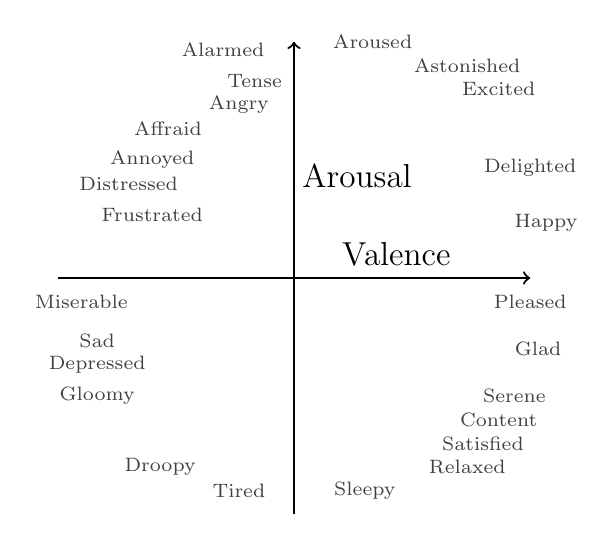
\begin{tikzpicture}
\large
\draw[thick,->] (3,0) -- (3,6) node[anchor=north east] {};
\draw[thick,->] (0,3) -- (6,3) node[anchor=north west] {};
\node at (3.8,4.3) {Arousal};
\node at (4.3,3.3) {Valence};

\scriptsize
\node[darkgray] at (4,6) {Aroused};
\node[darkgray] at (5.2,5.7) {Astonished};
\node[darkgray] at (5.6, 5.4) {Excited};
\node[darkgray] at (6, 4.4) {Delighted};
\node[darkgray] at (6.2, 3.7) {Happy};
\node[darkgray] at (6, 2.7) {Pleased};
\node[darkgray] at (6.1, 2.1) {Glad};
\node[darkgray] at (5.8, 1.5) {Serene};
\node[darkgray] at (5.6, 1.2) {Content};
\node[darkgray] at (5.4, 0.9) {Satisfied};
\node[darkgray] at (5.2, 0.6) {Relaxed};
\node[darkgray] at (3.9, 0.3) {Sleepy};
\node[darkgray] at (2.3, 0.3) {Tired};
\node[darkgray] at (1.3, 0.6) {Droopy};
\node[darkgray] at (0.5, 1.5) {Gloomy};
\node[darkgray] at (0.5, 1.9) {Depressed};
\node[darkgray] at (0.5, 2.2) {Sad};
\node[darkgray] at (0.3, 2.7) {Miserable};
\node[darkgray] at (1.2, 3.8) {Frustrated};
\node[darkgray] at (0.9, 4.2) {Distressed};
\node[darkgray] at (1.2, 4.5) {Annoyed};
\node[darkgray] at (1.4, 4.9) {Affraid};
\node[darkgray] at (2.3, 5.2) {Angry};
\node[darkgray] at (2.5, 5.5) {Tense};
\node[darkgray] at (2.1, 5.9) {Alarmed};
\end{tikzpicture}
\caption[Circumplex Model of Affect]{Circumplex Model of Affect \cite[S. 4]{8a02f9c512933d46fbea928d23ac65e38b61b88caba9b38319a5d4952b5a6667} bzw. \cite[S. 7]{russell1980circumplex}}
\end{figure}
\end{center}

Weiterhin sind Emotionen zu lesen, die an der entsprechenden Stelle im Valence-Arousal Koordinatensystem eingetragen sind \cite[S. 4]{8a02f9c512933d46fbea928d23ac65e38b61b88caba9b38319a5d4952b5a6667} \cite[S. 7]{russell1980circumplex}. Wie man sieht werden die abgebildeten Emotionen nach rechts hin glücklicher, sowie nach oben hin aufgeregter oder aktiver. Zu entscheiden ist nun, ob die Einteilung in Klassen oder die Approximation über ein Modell für eine Visualisierung besser geeignet ist.\\
Für die Umsetzung des Prototypen wurde das Circumplex Model of Affect benutzt, da ein Modell ein differenzierteres Ergebnis liefert, als die Klassifizierung. Auch könnten Fehler bei der Klassifizierung eher zu auffallend unpassenden Visualisierungen führen. Der Hauptgrund liegt aber darin, dass sich die Musik und damit auch die durch sie erzeugte Stimmung über die Zeit ändert \cite{8a02f9c512933d46fbea928d23ac65e38b61b88caba9b38319a5d4952b5a6667}. Diese Veränderungen lassen sich nur schwer über Klassen darstellen, da keine Möglichkeiten zwischen den Klassen existieren. Diese Veränderungen sind leicht über ein Modell zu realisieren, da zwischen zwei Punkten im Valence-Arousal-Raum beliebig viele Zwischenpunkte zu finden sind. Aus diesen Gründen werden zu den kontinuierlichen Daten ein Valence, sowie ein Arousal Wert hinzugefügt. Die praktische Berechnung dieser Werte wird im Abschnitt Implementierung behandelt.

\subsection{Zeit in der Musik}
Musik verändert sich über die Zeit. Aus diesem Grund ist es nicht zielführend einem Attribut der Musik einen einzelnen Wert pro Musikstück zu geben, sondern es ist vielmehr sinnvoll die Attribute und deren Entwicklung über die Zeit des Stückes zu betrachten. Würde man beispielsweise versuchen einen einzelnen Arousal-Wert zu errechnen, so würden ruhigere oder lautere Stellen nicht unterschiedlich visualisiert werden. Auch klingen gleiche Akkorde unterschiedlichen, wenn man sie in anderen Kontexten benutzt und sind somit Kontextabhängig. Die Emotionen verändern sich nicht sprunghaft, sondern entwickeln sich während des Hörens. Auch spielen Gedächtnis und Erwartung des Hörers eine entscheidende Rolle bei der Wahrnehmung von Musik \cite[S. 2]{8a02f9c512933d46fbea928d23ac65e38b61b88caba9b38319a5d4952b5a6667}. Aus diesen Gründen sind Durchschnittswerte von den gewonnenen Daten für eine Visualisierung uninteressant.\\
Um die Informationen in der Musik speichern zu können, wird eine passende Darstellung benötigt. Diese muss zu unterschiedlichen Zeitpunkten unterschiedliche Werte für das gleiche Attribut annehmen können. Bei der Umsetzung des Prototypen wurde diese zeitliche Darstellung für Events und kontinuierliche Daten unterschiedlich vorgenommen. Events besitzen, wie oben angesprochen ein Zeitattribut in Sekunden. Dadurch lassen sich Events auch nach Zeit sortieren, was für die Verarbeitung dieser hilfreich ist. Im Gegensatz dazu besitzen die kontinuierlichen Daten keine explizite Zeitangabe. Für die Umsetzung des Prototypen wurde die Musik in sogenannte Frames eingeteilt. Ein Frame ist eine Zeitspanne von 2048 Samples, was bei einer Samplerate von 44100 Hz einer Zeit von ca. 46.4 Millisekunden entspricht. Diese Frames überlappen sich zur Hälfte, was dazu führt, dass alle 1024 Samples (= 23.3 Millisekunden) ein Frame beginnt. Die Werte der kontinuierlichen Daten werden für jeden Frame neu berechnet und gespeichert, um für weitere Berechnungen zur Verfügung zu stehen oder für die Visualisierung benutzt zu werden.\\
Für die Einteilung in Frames bietet Essentia den ``FrameCutter'' Algorithmus \cite{EssentiaFrameCutter}. Von diesem lässt sich die Größe (FrameSize) als auch die Sprungweite (HopSize) konfigurieren. Alle weiteren kontinuierlichen Berechnungen bauen auf den so gewonnenen Frames auf.

\subsection{Visualisierung}
Will man eine 3D-Visualisierung umsetzen, so bietet es sich an Objekte zu benutzen, die passend zur Musik Eigenschaften 
und damit ihr Aussehen verändern. Position, Farbe und Form sind solche Eigenschaften. Über die Position selbst lassen sich wenig Informationen zum Betrachter transportieren, weshalb hier eher die Veränderung der Position, also die Bewegung, eine entscheidende Rolle spielt. Im Folgenden werden die einzelnen Attribute und ihre Verbindung zur Musik behandelt. Dadurch werden Möglichkeiten entwickelt, wie eine Visualisierung der vorher gewonnenen Daten umgesetzt werden kann.

\subsubsection{Farbe}
Der Zusammenhang von Musik und Farben ist wenig erforscht. Besser erforscht ist hingegen der Zusammenhang zwischen Farben und Emotionen, so werden Farben bewusst eingesetzt, um in Bildern, Filmen, Computerspielen und anderen Multimediaanwendungen gesteuerte Emotionen hervorzurufen \cite{10.3389/fpsyg.2017.00440}. Will man menschliche Emotionen untersuchen, so werden häufig kurze Filme oder Bilder verwendet, um die gewünschten Emotionen zu erzeugen. Zu beachten ist hierbei, dass gleiche Farben in unterschiedlichen Ländern und Kulturen unterschiedliche Bedeutungen haben und dadurch unterschiedliche Emotionen hervorrufen können. So ist in China die Farbe des Todes Weiß, während es in westlichen Ländern Schwarz ist.\\
In Tabelle 3 sind Farben und ihre nach Naz Kaya and Helen H. Epps
 \cite{c0f471f7e6a618d880cf25175c9f99ac97ef8ba7d016c7f8c523f8d902892d9e} zugeordneten Emotionen und Assoziationen zu sehen.

\definecolor{yellow_color}{RGB}{248, 230, 77}
\definecolor{green_color}{RGB}{0, 142, 78}
\definecolor{blue_color}{RGB}{5, 158, 212}
\definecolor{red_color}{RGB}{218, 65, 74}
\definecolor{white_color}{RGB}{255, 255, 255}
\definecolor{gray_color}{RGB}{80, 80, 80}
\definecolor{black_color}{RGB}{0, 0, 0}

\begin{center}
\begin{table}[h!]
\begin{tabular}{l | l | l | l}
\textbf{Farbe} & & \textbf{Emotionen} & \textbf{Assoziationen}\\
\hline
Gelb & \cellcolor{yellow_color} & Fröhlichkeit, Aufregung & Sonne, Sommer \\
Grün & \cellcolor{green_color} & Fröhlichkeit, Entspannung, Frieden, Hoffnung & Natur, Pflanzen \\
Blau & \cellcolor{blue_color} & Ruhe, Entspannung & Ozean, Himmel \\
Rot & \cellcolor{red_color} & Liebe, Wärme, Aktivität, Gefahr & Herzen, Blut \\
Weiß & \cellcolor{white_color} & Unschuld, Friede, Einsamkeit, Langeweile & Brautkleid, Schnee \\
Grau & \cellcolor{gray_color} & Traurigkeit, Langeweile & Schlechtes Wetter \\
Schwarz & \cellcolor{black_color} & Depression, Angst & Trauer, Wohlstand \\

\end{tabular}
\captionsetup{justification=centering}
\caption[Farben Emotionen Assoziationen]{Farben, ihre Emotionen und Assoziationen\\nach Naz Kaya and Helen H. Epps
 \cite{c0f471f7e6a618d880cf25175c9f99ac97ef8ba7d016c7f8c523f8d902892d9e}}

\end{table}
\end{center}
Trägt man die Farben entsprechend den Beschreibungen in ein Valence Arousal Koordinatensystem ein, so ergibt sich der in Abbildung 5 zu sehende Verlauf.

\begin{wrapfigure}{l}{0.5\linewidth}
\begin{tikzpicture}[]
  \pgftext{\includegraphics[scale=0.5]{res/images/color_map}} at (0pt,0pt);
  \draw[white,thick,->] (-3,-3) -- (-3,3) node[anchor=north west] at(-3, 1) {Arousal};
  \draw[white,thick,->] (-3,-3) -- (3,-3) node[anchor=north east] at(1, -3) {Valence};
\end{tikzpicture}
\captionsetup{justification=centering}
\caption[Farbverlauf im Valence Arousal Koordinatensystem]{Farbverlauf\\im Valence Arousal\\Koordinatensystem}
\end{wrapfigure}
\noindent
Jedem Punkt im Arousal Valence Koordinatensystem ist eine entsprechende Farbe zugeordnet. Bei niedrigen Arousal Werten, also bei ruhiger Musik, gehen die Farben ins Blaue beziehungsweise ins Graue für kleine Valence Werte oder ins Grüne für hohe Valence Werte. Gelbe Farben werden bei aktiven fröhlichen (hohe Valence und hohe Arousal Werte) erzeugt und rote Farben, wenn die Musik weniger fröhlich, aber immer noch aktiv ist. Wird die Musik noch trauriger wird Schwarz erzeugt. In der Mitte befindet sich ein Orange-Braun. Dies ist nur eine mögliche Anordnung von Farben und es würde sich eventuell anbieten, weitere kompatible Farbeverläufe zu kreieren, um Farbkombinationen zu ermöglichen. Die Umsetzung der Stimmung$ \rightarrow $Farbe-Zuordnung wird im Kapitel Implementierung behandelt.

\subsubsection{Bewegung}
Bewegung und Musik sind eng miteinander verbunden. Rolf Inge God{\o}y und Alexander Refsum Jensenius meinen: ``Performers produce sound through movements, and listeners very often move to music, as can be seen in dance and innumerable everyday listening situations.'' \cite[S. 1]{905eee055abaf2a4f198ce11f35362a8963f61d552297a02dfc8fbc0c4f78679}. Aus diesem Grund ist die Auswahl von Bewegungen für eine Visualisierung wichtig. Im Folgenden werden erst Grundprinzipien natürlicher Bewegungen besprochen. Danach Parameter von Bewegungen und warum diese für die Visualisierung wichtig sind. Zum Schluss werden beispielhaft bestimmte Typen von Bewegungen und Formationen besprochen.
\paragraph{Grundprinzipien}
In der Umwelt sind physische Dinge massebehaftet. Daraus folgt, dass es weder schlagartige Positions- noch Geschwindigkeitsänderungen gibt. Will man eine Gruppe von Objekten oder Partikeln natürlich bewegen, so muss dieser Fakt mit einbezogen werden. Angenommen wird hierbei meistens eine Punktmasse, wobei die gesamte Masse des Objektes im Zentrum des Objektes liegt. Dadurch werden die Bewegungen des Objektes besser berechenbar.\\
Um plötzliche Positions- und Geschwindigkeitsunterschiede zu vermeiden sollten bewegte Objekte eine persistente Position und eine persistente Geschwindigkeit haben, die jeden Frame verändert werden kann. Auf die Position wird die Geschwindigkeit addiert. Eine Wirkung auf das sich bewegende Objekt erzeugt man durch Beschleunigungen, welche die aktuelle Geschwindigkeit anpassen. Diese Beschleunigungen können plötzlich auftreten und werden jeden Frame neu berechnet. Sie sind also nicht über mehrere Frames persistent wie die Position oder die Geschwindigkeit.\\
Eine bekannte Methode, um Objekte natürlich zu beschleunigen ist das sogenannte ``Steering Behaviour'' \cite{580abc6c6615ef9f9c16f9069351938a0dda3c5120b7e8d1450d6b1abf0a71df}. Dabei wird eine Beschleunigung für ein bewegtes System errechnet. Das Ziel ist es das Objekt zu einem gewissen Punkt zu bringen oder es davon zu entfernen. Es gibt mehrere Variationen des Steering Behaviours, es soll hier aber nur um die einfache Form ``Seek'' (Anstreben) gehen.\\
Hat ein bewegtes System die Geschwindigkeit $current\_velocity$, eine maximale Geschwindigkeit von $max\_velocity$ und die Position $current\_position$ und existiert weiterhin ein angestrebter Punkt $target\_position$, so kann man eine einwirkende Beschleunigung $steering\_force$ berechnen, die das Objekt zur $target\_position$ bringt.
\begin{align}
desired\_velocity &= current\_position - target\_position \\
steering\_force &= desired\_velocity - current\_velocity
\end{align}
Neben dem Seek Algorithmus gibt es Abwandlungen, wie ``Flee'', ``Arrive'' oder ``Wander''.\\
Um die Geschwindigkeit zu begrenzen kann Formel (1) wie folgt abgewandelt werden:
\begin{align}
desired\_velocity &= (current\_position - target\_position) * max\_velocity
\end{align}
\noindent
Die Formel (2) bleibt bestehen.\\
Eine andere Möglichkeit die Geschwindigkeit zu begrenzen, ist es eine Reibung (einen Drag) einzuführen. Dazu wird die Geschwindigkeit mit folgender Beschleunigung addiert:
\begin{align}
drag\_force = current\_velocity * -drag
\end{align}

\noindent
Die Variable $drag$ sollte dabei eine Zahl $0 < drag < 1$ sein. Ein kleiner $drag$ bedeutet eine geringe Dämpfung, während ein großer $drag$ eine stärkere Dämpfung der Geschwindigkeit erzeugt.

\paragraph{Bewegungen spannend gestalten}
Eine Bewegung von Objekten sollte möglichst nicht einseitig werden, weshalb ein zufälliger Anteil der Abläufe vorteilhaft sein kann. Eine andere Möglichkeit, um die entstehenden Bilder abwechslungsreich zu gestalten, ist Parameter der Bewegungen zu definieren, die abhängig von den analysierten Daten verändert werden können. Nicht alle Parameter müssen von allen Bewegungen implementiert werden.\\
Die Geschwindigkeit der bewegten Objekte kann als Parameter verwendet werden. Aktive, hektische Musik kann auf diese Weise behandelt werden, indem die Geschwindigkeit der Objekte erhöht wird. Unter Umständen bietet es sich bei Gruppenbewegungen an, einen Parameter einzuführen, der beschreibt, wie kompakt die Objekte beieinander gehalten werden und einen Parameter, der beschreibt, wie häufig sich Richtungsänderungen der Bewegungen ereignen.\\

\paragraph{Mögliche Bewegungen}
Im Folgenden sollen Beispiele für Bewegungen beleuchtet und darauf untersucht werden, ob sie sich für eine Visualisierung eignen. Dazu wird geprüft, ob die Bewegung interessant genug ist und ob sie sich performant genug umsetzen lässt.\\

\begin{itemize}
\item \textbf{Flow Fields:} Flow Fields sind eine interessante Art der Bewegung, die in der Computergraphik vor allem für die Simulation von Flüssigkeiten eingesetzt werden \cite{stam1999stable}. Sie stellen ein in Quadrate eingeteilten Raum dar. Für jedes Quadrat wird ein zufälliger Vektor bestimmt, der sich den Vektoren der umliegenden Quadrate ähnelt. Nun werden Partikel in diesem Raum erzeugt. Der Mittelpunkt von jedem Partikel befindet sich in genau einem der Quadrate. Jeder Partikel wird in Richtung des Vektors beschleunigt, in dessen zugehörigen Quadrat er sich befindet. Durch die Ähnlichkeit der Vektoren von anliegenden Quadraten entsteht eine Fließbewegung der Partikel. Eine Erweiterung wäre, die Vektoren der Quadrate über Zeit verändern zu lassen, um die Bahnen der Partikel zu verändern. Auch kann die Beschleunigung der Partikel verändert werden, sowie die Kompaktheit des Feldes.\\
Die Umsetzung eines Flow Fields ist aufwendig, da es nicht einfach ist, den Anforderungen entsprechende Richtungsvektoren zu generieren, die sich über Zeit verändern und dabei ihre Ähnlichkeit bewahren. Um diese Vektoren zu generieren, wird ``Perlin Noise'' oder der Nachfolger ``Simplex Noise'' verwendet \cite{bcc7190da8e90284b4e790817b8eed4ee3ea6cffbe5a23ef07a000ca5628ffbc}. Perlin Noise ist eine Zufallsfunktion mit besonderen Eigenschaften. Sie wurde 1982 von Ken Perlin für den Film ``Tron'' entwickelt. Perlin erhielt dafür 1997 einen Oscar.\\
Perlin Noise ist eine kontinuierliche Funktion, die im  eindimensionalen Fall eine Zahl $x \in \mathbb{R}$ auf eine andere zufällige Zahl $noise(x) \in \mathbb{R}$ abbildet \cite{25a05da283ffd9d4bdda94c308ccf3a8759f22373b368f895cbef2e9186ab646}. Weiterhin sorgt eine kleine Änderung von $x$ auch nur für eine kleine Änderung von $noise(x)$. Ein möglicher Plot der Perlin Noise Funktion ist in Abbildung 6 zu sehen.
\begin{SCfigure}[][h]
\hspace{110pt}
\includegraphics[scale=0.5]{res/images/perlin_noise}
\caption[Perlin Noise Plot aus \cite{nature_of_code}]{\\Perlin Noise Plot aus \cite[\\Kap. Introduction]{nature_of_code}}
\end{SCfigure}
\end{itemize}

Weiterschreiben...

\newpage
\subsubsection{Größe}

\newpage

\section{Implementierung / Umsetzung}
\subsection{Grobe Aufteilung}
Visualizer (OpenGL) / AudioVisualizer / Essentia
\subsection{Visualizer}
\paragraph{OpenGL}
\paragraph{Shapes}
\paragraph{Entities}
\paragraph{Movements}
\paragraph{Creations}
\paragraph{Queries}
\subsection{AudioVisualizer}
\paragraph{DataGenerators}
\subparagraph{Die implementierten DataGenerators}
\paragraph{EventGenerators}
\paragraph{Dependencies}
\paragraph{Handler}
\paragraph{EventSystem}
\paragraph{Essentia}
\paragraph{Compositor}

\section{Fazit}
Auf Anforderungen eingehen
\subsection{Erlebnis}

\newpage

\bibliography{bib/literatur}
\bibliographystyle{alpha}

\listoftables
\listoffigures

\end{document}
